\subsection{Modelle}

\hfill \break
Lineares Modell:\\
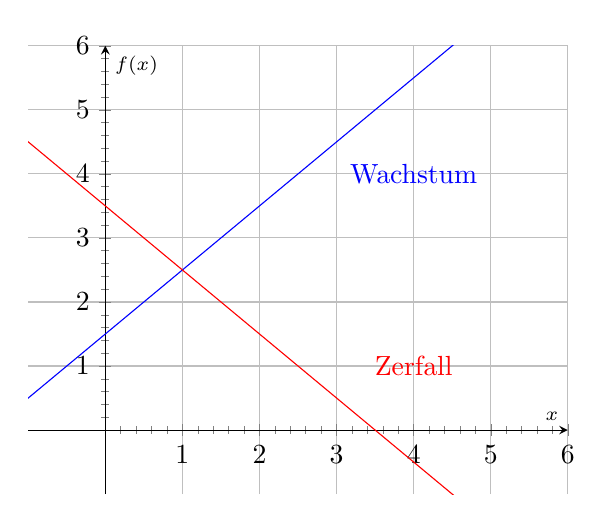
\begin{tikzpicture}[scale=1.0]
    \begin{axis}%
        [
            grid=major,
            xtick={0,1,...,7},
            minor x tick num=4, % 4 minor ticks => 5 subintervals
            xmin=-1,
            xmax=6,
            xlabel={\scriptsize $x$},
            axis x line=middle,
            ytick={0,1,...,7},
            minor y tick num=4,  % 4 minor ticks => 5 subintervals
            ymin=-1,
            ymax=6,
            ylabel={\scriptsize $f(x)$},
            axis y line=middle,
            no markers,
            samples=100,
            domain=-6:6,
        ]
        \addplot[blue] (x,{x+1.5});
        \addplot[red] (x,{-x+3.5});
        \node[color=blue] at (4,4) {Wachstum};
        \node[color=red] at (4,1) {Zerfall};
    \end{axis}
\end{tikzpicture}

\hfill \break
Exponentielles Modell:\\
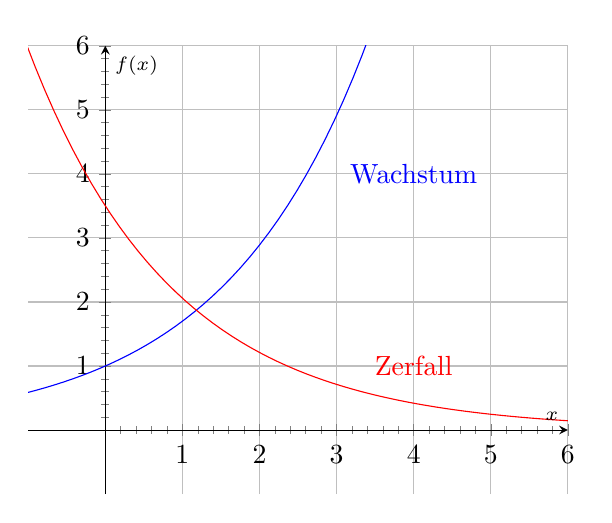
\begin{tikzpicture}[scale=1.0]
    \begin{axis}%
        [
            grid=major,
            xtick={0,1,...,7},
            minor x tick num=4, % 4 minor ticks => 5 subintervals
            xmin=-1,
            xmax=6,
            xlabel={\scriptsize $x$},
            axis x line=middle,
            ytick={0,1,...,7},
            minor y tick num=4,  % 4 minor ticks => 5 subintervals
            ymin=-1,
            ymax=6,
            ylabel={\scriptsize $f(x)$},
            axis y line=middle,
            no markers,
            samples=100,
            domain=-6:6,
        ]
        \addplot[blue] (x,{1.7^x});
        \addplot[red] (x,{3.5*(1.7^-x)});
        \node[color=blue] at (4,4) {Wachstum};
        \node[color=red] at (4,1) {Zerfall};
    \end{axis}
\end{tikzpicture}

\hfill \break
Beschränktes Wachstum:\\
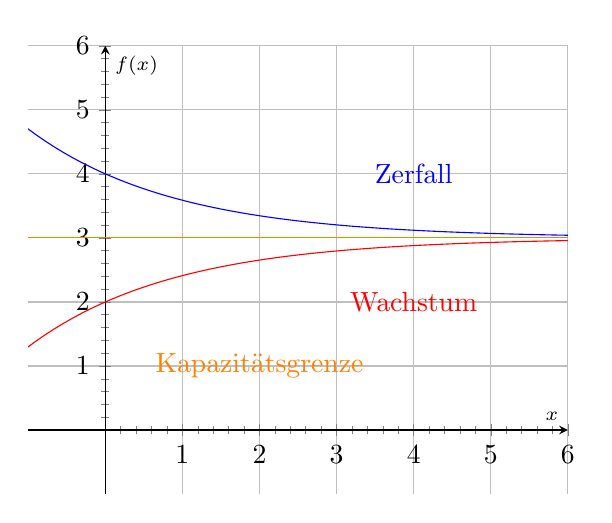
\begin{tikzpicture}[scale=1.0]
    \begin{axis}%
        [
            grid=major,
            xtick={0,1,...,7},
            minor x tick num=4, % 4 minor ticks => 5 subintervals
            xmin=-1,
            xmax=6,
            xlabel={\scriptsize $x$},
            axis x line=middle,
            ytick={0,1,...,7},
            minor y tick num=4,  % 4 minor ticks => 5 subintervals
            ymin=-1,
            ymax=6,
            ylabel={\scriptsize $f(x)$},
            axis y line=middle,
            no markers,
            samples=100,
            domain=-6:6,
        ]
        \addplot[blue] (x,{(1.7^-x)+3});
        \addplot[red] (x,{(-1.7^-x)+3});
        \node[color=blue] at (4,4) {Zerfall};
        \node[color=red] at (4,2) {Wachstum};
        \addplot[orange] (x,{3});
        \node[color=orange] at (2,1) {Kapazitätsgrenze};
    \end{axis}
\end{tikzpicture}

\hfill \break
Logisches Wachstum:\\
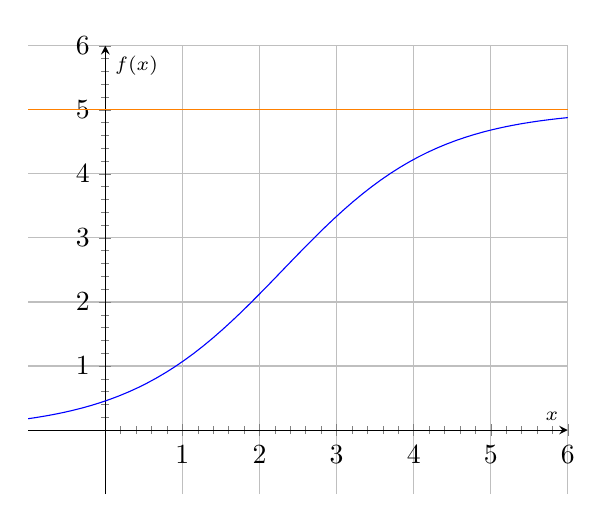
\begin{tikzpicture}[scale=1.0]
    \begin{axis}%
        [
            grid=major,
            xtick={0,1,...,7},
            minor x tick num=4, % 4 minor ticks => 5 subintervals
            xmin=-1,
            xmax=6,
            xlabel={\scriptsize $x$},
            axis x line=middle,
            ytick={0,1,...,7},
            minor y tick num=4,  % 4 minor ticks => 5 subintervals
            ymin=-1,
            ymax=6,
            ylabel={\scriptsize $f(x)$},
            axis y line=middle,
            no markers,
            samples=100,
            domain=-6:6,
        ]
        \addplot[orange] (x,{5});
        \addplot[blue] (x,{5/(1+10*e^-x)});
    \end{axis}
\end{tikzpicture}